\section{State of the Art}

Before the main matter of the thesis, it is important to expose the current
state of the art, to check if the previous research done in the topics
related to this project. First, the section will sum up the current state of
the art in the algorithms that will be used by the thesis, as well as all
naming several libraries currently used for that purpose. Last, this section
will provide a basic state of the language to be used, Haskell; that will also
serve as a motivation for why to develop the project using this tool.\\

\subsection{Heuristic Search}

Heuristic Search is a problem solving method that belongs to Artificial
Intelligence \cite{rusell-2003-aima} used in robotics, pathfinding, computer
gaming among other fields. We can distinguish two types of heuristic search
algorithms: uninformed algorithms, which do not use a heuristic function and
perform a brute-force search; and informed algorithms, which use a heuristic
function to provide better performance than the aforementioned brute-force
algorithms.\\

\begin{figure}[ht]
\centering
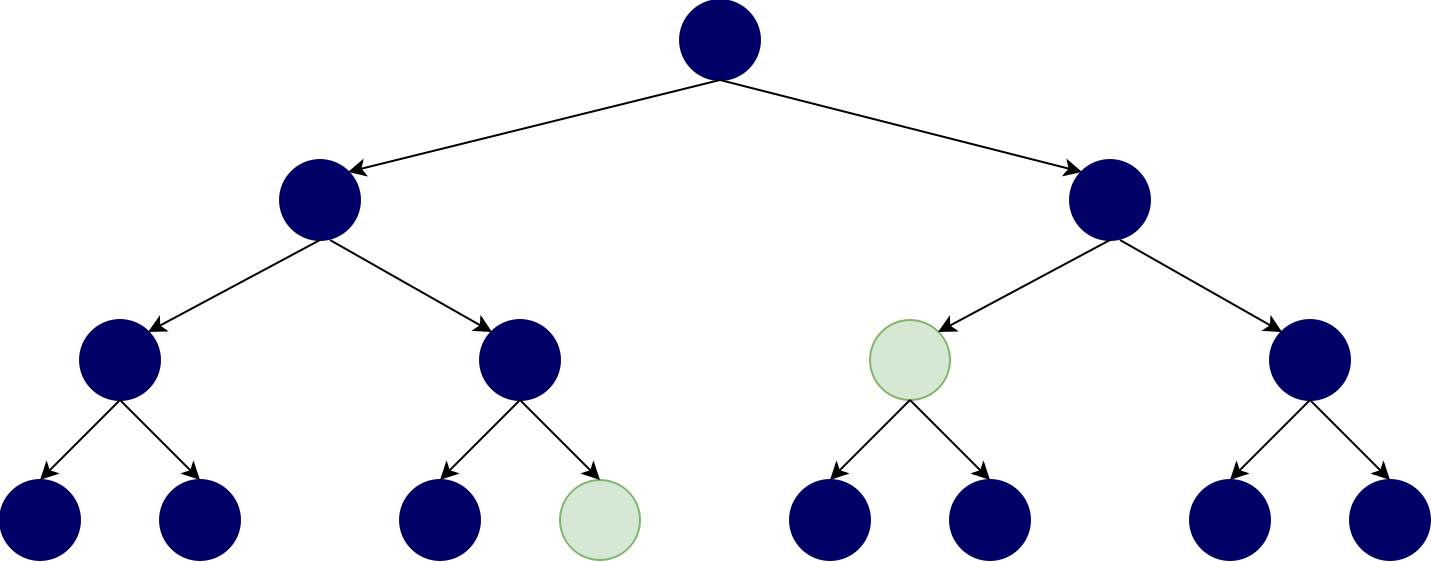
\includegraphics[width=0.8\textwidth]{img/empty-tree.png}
\caption{Example of a search tree}
\label{tree:empty}
\end{figure}

Although every algorithm included in this thesis can work with implicit graphs,
the best way to gain some intuition about them is to reflect their behavior on
a search tree, like the one in Figure \ref{tree:empty}. This tree presents a
root node (top of the image), from which is possible to see two different
oriented edges going out to two new nodes. This presents in a explicit way the
fact of being able to traverse the search space using operators given in a
problem space. The green nodes present final states. The objective of any
search algorithm then is to find a path from the root node (which is the
initial state defined in the problem space) to a final node, using different
constraints depending on the problem at hand: the shortest path, lowest cost
path, or just a solution that can be found in the shortest time possible. Using
this graphical representation, we can now go deep into explaining the current
state of the art of the algorithms that will be included in the framework.\\

\subsubsection{Uninformed Algorithms}

One of the basic brute-force algorithms is, undoubtedly, Breadth-First Search.
It was first introduced by Konrad Zuse in 1945, although published years later
\cite{zuse-1972-plankalkul}. This algorithm uses a queue (First In, First Out)
data structure to store the nodes expanded. The use of this queue to sort the
nodes to expand results in an exhaustive search per depth in the tree: first
the depth 0 nodes are expanded, the depth 1, the depth 2, etc, until the
solution is found or until the search space is completely exhausted. This
behavior can be appreciated in Figure \ref{tree:bfs}.\\

\begin{figure}[ht]
\centering
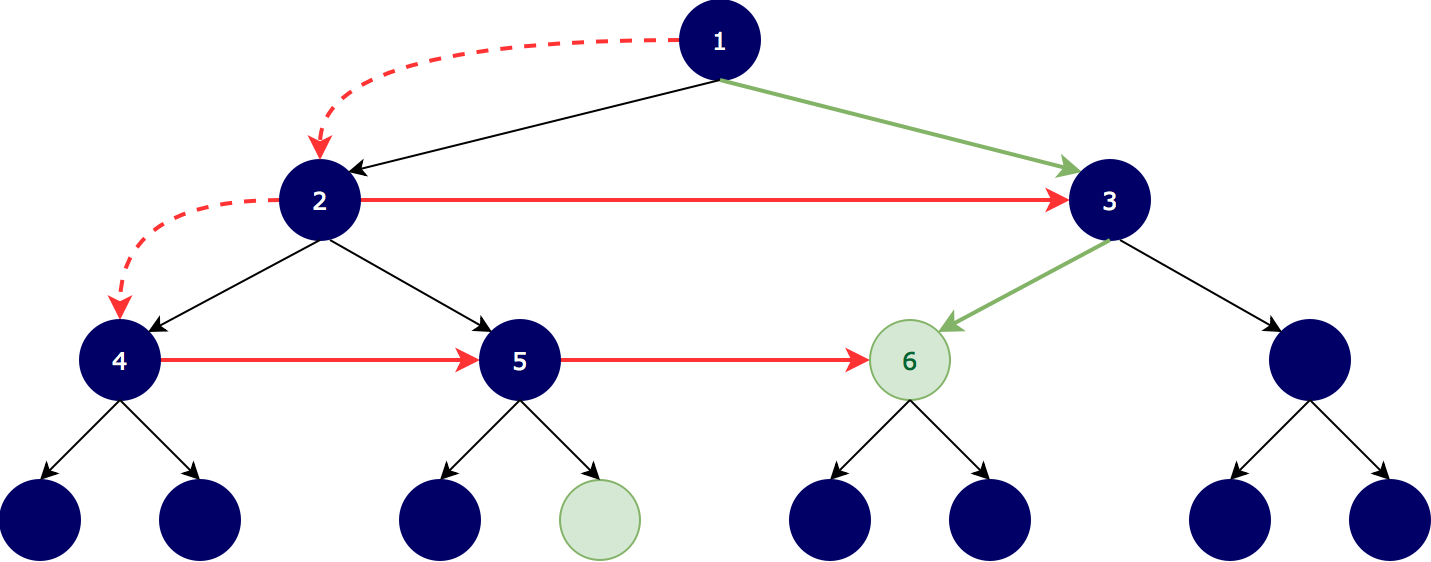
\includegraphics[width=0.8\textwidth]{img/bfs.png}
\caption{Breadth-First Search execution on the tree}
\label{tree:bfs}
\end{figure}

In Figure \ref{tree:bfs} it is possible to see that the nodes are visited from
shallower to deeper levels, ensuring that the solution returned by this
algorithm is indeed the one with the shortest path from the initial state. The
algorithm is complete, that is, it will find a solution if it exists in the
search space, even if such space is infinite. The solution found will be the
nearest to the initial state, which is ensured to be the optimal if there no
variable costs. Its complexity is defined by $O(|V|)$, that is, the total
number of states. This is common to all search algorithms: theoretically, they
have to check all states in a worst case scenario. However, it is important to
notice that the complexity to finding a certain solution at a depth $d$ is
$O(b^{d+1})$, where $b$ is the branching factor of the problem
\cite{rusell-2003-aima}.\\

Another well-known uninformed algorithm is Depth-First Search. This algorithm
uses the opposite approach to the problem: tries to search as deep as possible
before exhausting a branch or finding a solution. This algorithm was first
studied by Charles Pierre Trémaux in the 19th Century, with the purpose of
solving mazes with well defined passages \cite{even-2011-graph}. This algorithm
does not need a auxiliary data structure to hold nodes: instead, it is possible
to explore the nodes in depth just using recursive calls to the algorithm. This
allows Depth-First Search to perform searches in linear space, since it only
needs to store the stack calls needed to keep track of the search. Although
this is convenient for this project, it is possible as well to use a stack
structure (Last In, First Out) to hold all the nodes in an imperative language
in case the recursion is not desired \cite{rusell-2003-aima}. A complete
execution of this algorithm can be found in Figure \ref{tree:dfs}\\

\begin{figure}[ht]
\centering
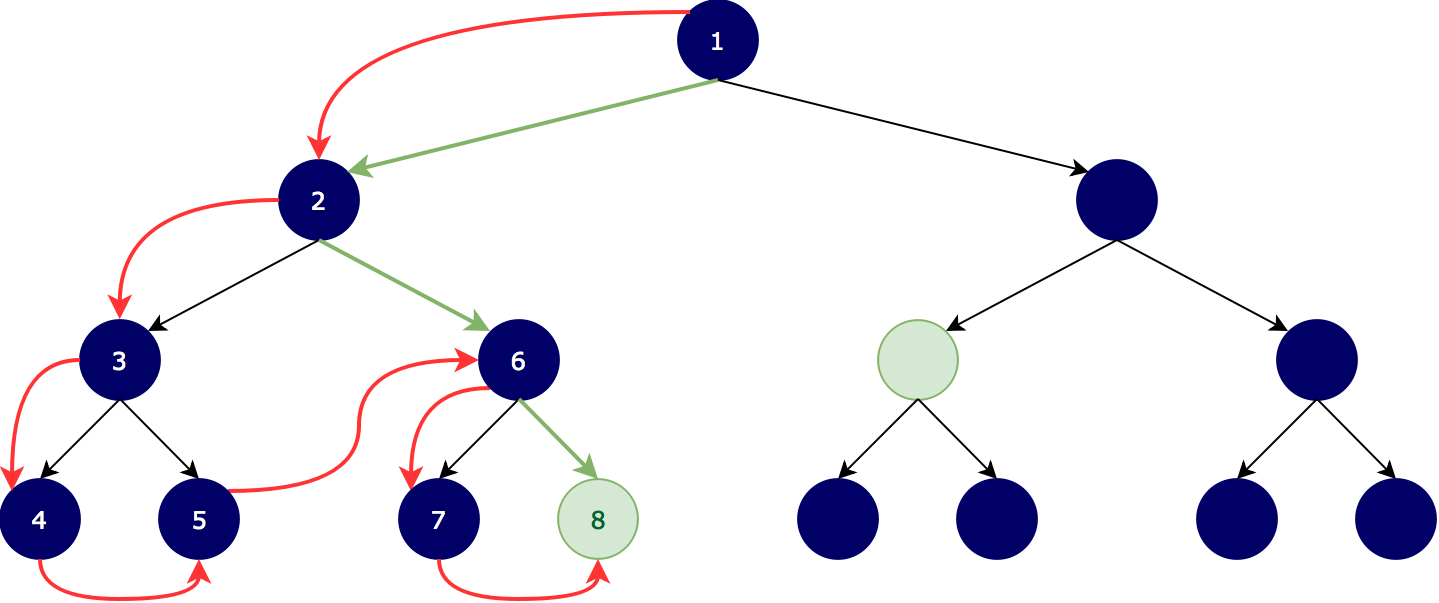
\includegraphics[width=0.8\textwidth]{img/dfs.png}
\caption{Depth-First Search execution on the tree}
\label{tree:dfs}
\end{figure}

In the execution of Figure \ref{tree:dfs}, it is possible to see how it
exhausts the first branch until no more nodes can be expanded, to then
backtrack. This backtracking can be implicitly implemented (by using recursive
calls it is possible to recover from an exhausted branch). We can see how this
search returns a worse solution than Breadth-First: the solution found by the
algorithm is 3 operations away from the initial state, while the existing
solution found before has been completely ignored by this algorithm. The main
advantage of this algorithm is its space complexity to find a given solution at
a depth $d$ is indeed linear, and its execution to find a solution should
average faster than Breadth-First Search \cite{zhang-1995-bnb}. However,
Depth-First Search is not complete in implicit graphs: since the depth of the
tree can be infinite, the search can get lost expanding nodes that do not lead
to a recursion \cite{rusell-2003-aima}.\\

For that reason, the Iterative-Deepening Depth-First Search was developed: by
limiting the depth at which a Depth-First algorithm can explore, the
backtracking is used to explore certain depths \cite{korf-1985-depth}. This
eliminates the lack of completeness, and makes IDDFS equivalent to a
Breadth-First Search if the step used to increase the depth bound is one. It is
however important to remark that this algorithm is faster than BFS in the last
iteration but most likely slower if taking into account the cumulative time of
all depth executions. Its time and space complexity are the same of Depth-First
Search, but it is complete and optimal if the depth is increased one by one.\\

The last uninformed algorithm to explore is Uniform Cost Search. This algorithm
performs a brute-force search expanding first the lowest-cost node, using a
BFS-like fashion to explore the search space \cite{rusell-2003-aima}. This
algorithm is sometimes referred to as Dijkstra's Algorithm, although the latter
is considered to be subtly different and since we are applying it to implicit
graphs, the algorithm will be treated as UCS along the thesis
\cite{felner-2011-dijkstra}. This algorithm relies on a priority queue that
sorts the nodes and always returns the one whose current cost is lower. For
that reason, Uniform Cost Search can be seen as a variation of Breadth-First
Search that takes into account variable cost paths and thus always return the
lowest cost solution, instead the shorter one. UCS is, therefore, complete and
optimal.\\

\subsubsection{Informed Algorithms}

Informed algorithms are those that perform searches using a heuristic function.
This function evaluates a state and returns a value that presents how close
that state is to a solution. Using those values, the states can be ranked on
how convenient they are for the search (the closer to the solution, the more
relevant to the search is to expand such state) \cite{pearl-1984-heuristics}.\\

The main informed algorithm to take into account is the well-known A*
algorithm. First developed in 1968 as an extension of Dijkstra's algorithm, it
features an evaluation function that takes into account both the cost of a node
and its heuristic value \cite{hart-1968-formal}. The algorithm uses a priority
queue to sort the nodes in ascending order of $f$, the aforementioned
evaluation function. This function is defined as $f(n) = g(n) + h(n)$ where $g$
is the cost of the node and $h$ is the value of the heuristic function. That
way, the algorithm expands the nodes keeping a balance of current and expected
cost to obtain the solution. Two examples of this algorithm can be found in
Figure \ref{tree:astar}.\\

\begin{figure}[ht]
\centering
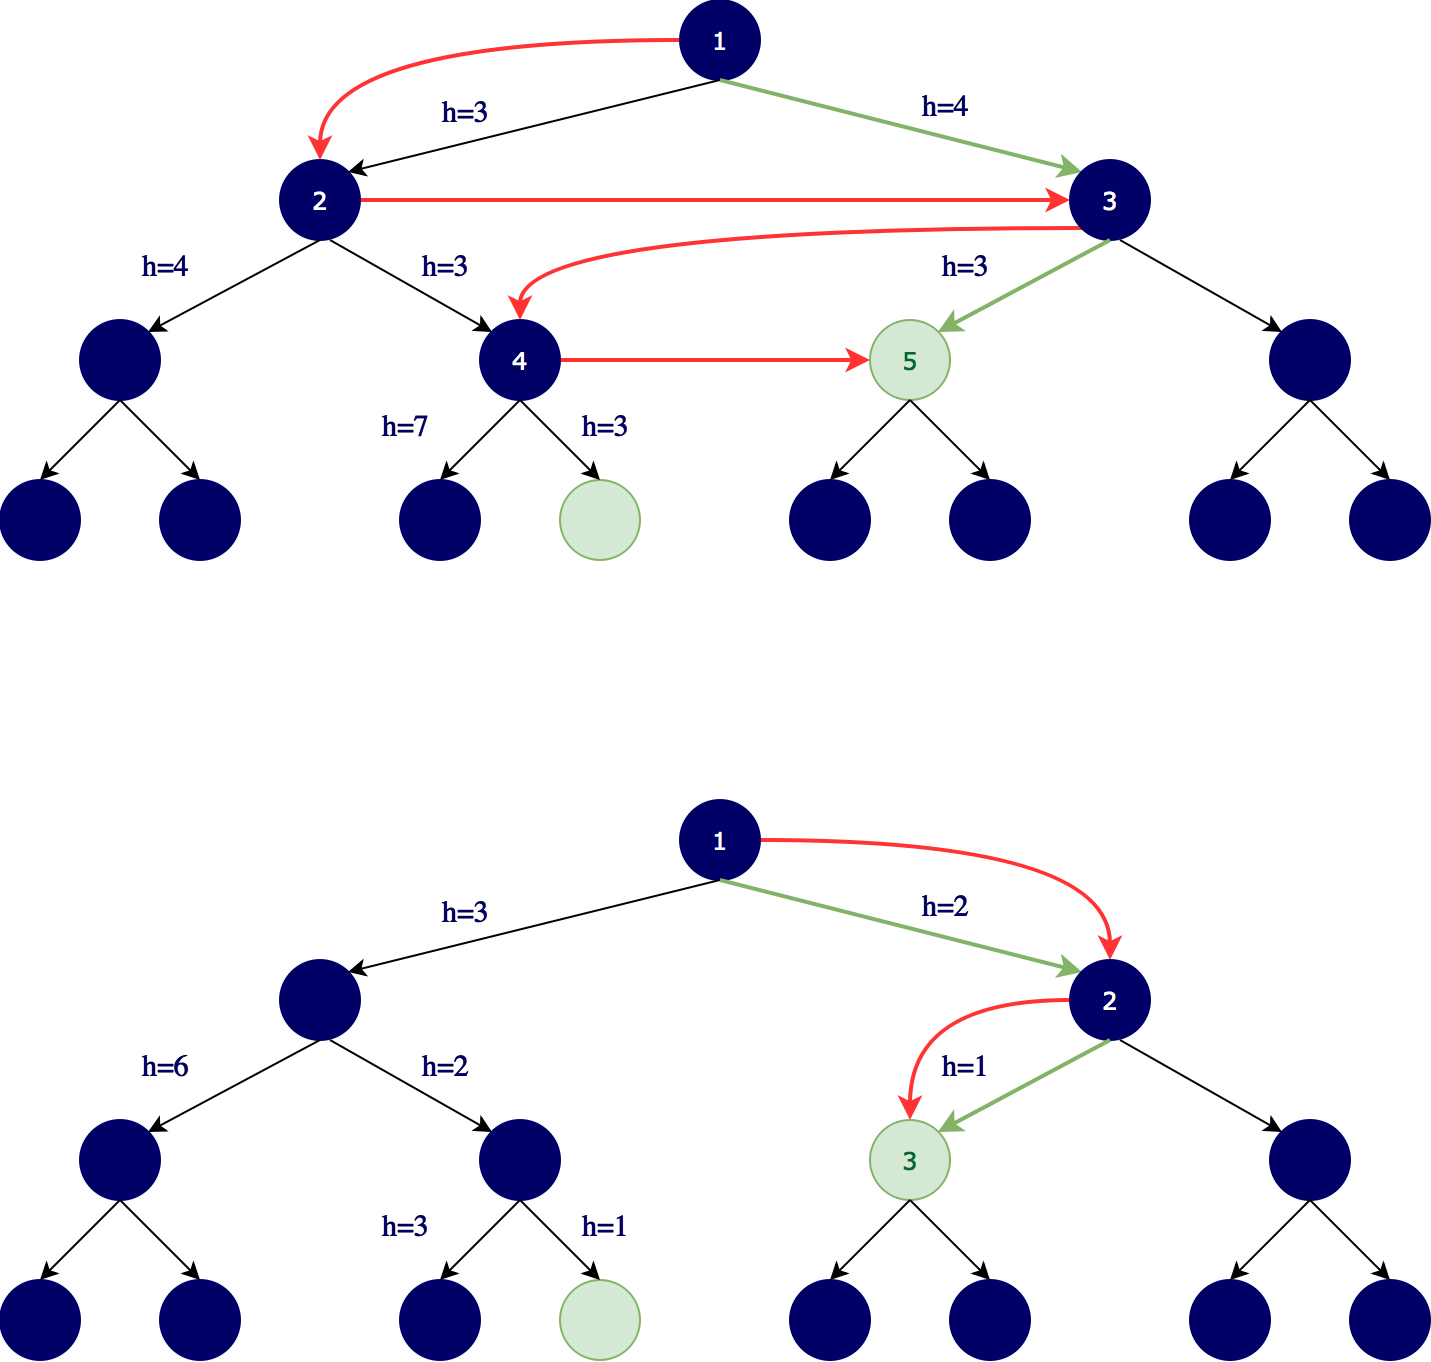
\includegraphics[width=0.8\textwidth]{img/astar.png}
\caption{A* Search executions using two different heuristics}
\label{tree:astar}
\end{figure}

In the first execution of Figure \ref{tree:astar} shows how the nodes are
expanded using the values computed at each iteration. At each new iteration,
the branch expanded is the one with lower projected costs. In the second
execution, we can see how a different heuristic returns the same solution but
expanding less nodes. This introduces an important concept of A*: with a
perfect heuristic, A* performs a perfect search, expanding only the necessary
nodes to obtain and ensure that the solution found is optimal
\cite{dechter-1985-astar}. This implies that the heuristic is relevant for the
node performance, but not only that: A* is only complete and optimal if the
heuristic function used is admissible, that is, if it never underestimates the
actual cost of getting from a node to a solution \cite{pearl-1984-heuristics}.
Its complexity in worst case scenario is the one of Breadth-First Search;
$O(b^{d+1})$.\\

Following a similar idea, but using iterative-deepening for obtaining a better
memory performance, it is important to mention Iterative-Deepening A*
\cite{korf-1985-depth}. The basic idea behind it is to perform a depth-first
search using the $f$ function of A*. This results in a linear-memory algorithm,
that explores the solutions in thresholds defined by $f$ as a cutoff function.
This makes an interesting algorithm when memory constraints exist, and it is
ensured to return the shortest path from the initial state to a solution as
long as the heuristic is admissible.\\
\subsubsection{Libraries}

Due to being more appropriate for the performance that is in general desired,
we can find that the most amount of work on Heuristic Search is done in
imperative, fast languages like C++ or Java.\\

In C++, we can find full search frameworks like \emph{HOG2} \cite{hog2},
\emph{Research code for heuristic search} \cite{cpp-search} or \emph{The
  Heuristic Search Research Framework} \cite{goldenberg-2017-framework}. All
these frameworks offer a full set of algorithms and procedures to override the
default implementations (such as cost, heuristic or expansion functions) in
order to adapt the library's behavior to the problem at hand. Also, these
frameworks offer visual representations options; a feature which is indeed the
main goal in the case of \emph{The Heuristic Search Research Framework}, that
offers a general visualization of algorithm behavior instead of domain specific
ones. On the other hand, in Java we can find similar projects like
\emph{Combinatorial Search for Java} \cite{cs4j} or \emph{AIMA}
\cite{java-aima}.\\

Trying to find similar projects in functional languages is more complicated
than that. However, one can find interesting projects like \emph{AIMA} written
in Common Lisp \cite{lisp-aima} or even a complete search framework written in
OCaml \cite{ocaml-search}. In Haskell, however, projects of this size are
nowhere to be found: All the algorithms are distributed in individual packages
with completely different implementations, as well as the data structures used
to perform the search.


\subsection{Haskell}

Haskell's first version was released in 1990 after the efforts of a committee
in FPCA '87 for creating an open standard for a ``non-strict, purely functional
language'' \cite{haskell-history}. Haskell's main features have remain patent
in the language, but constantly evolving: the language's main pillars are
\cite{haskell-98, haskell-2010}:

\begin{enumerate}
\item \textbf{Strong and statically typed}: the types are checked at compile
  time. That makes the run-time be sure that every function will get as
  parameter the expected object, making it more robust. However, no explicit
  type declaration is needed (although it is usually considered a good
  practice); types can be inferred most of the times by the compiler.
\item \textbf{Purely functional}: this type system is what allows Haskell to be
  purely functional. For Haskell, a string literal is of type \texttt{String},
  while an user's input on the prompt is a \texttt{IO String}. While at first
  shocking, this quality of Haskell maintains the referential transparency
  intact: the same function call with the same arguments is guaranteed to
  provide always the same output. All side effects are contained into monads
  (like the aforementioned \texttt{IO} monad) so they are contained and
  isolated.
\item \textbf{Lazy}: the fact that Haskell's evaluation is lazy (contrary to
  more common strict evaluation) means that a expression is only computed if
  its result is really necessary at a moment in time. This allows expressions
  to be defined in a much higher level: telling the computer what something is
  rather than how to compute it, and leaving the details of it to the compiler.
  Lazy evaluation provides for instance the use of infinite lists (since only
  the necessary part will be actually evaluated).
\item \textbf{Concurrent abstractions}: All the aforementioned characteristics
  also add up to the fact that the compiler is able to include concurrent
  optimizations into regular Haskell code thanks to its high-level definitions.
\end{enumerate}

Currently, the Glasgow Haskell Compiler (GHC) can be almost considered the
de-facto standard in Haskell compilers: widely spread and with an impressive
interface of pragmas to enable different optimizations by the compiler, it is
the compiler used for most projects because of the language extensions it
provides. Regarding packaging frameworks we can use Cabal, as a more
established option; or Stack, that wraps around Cabal configurations offering
more robust dependency installs and builds. Both frameworks offer several tools
for compilation, packaging, documentation, distribution, testing and profiling.
These tools will be explained in detail as they appear in the thesis.\\

Although not yet mainstream, Haskell is a language used in the industry that is
specially well-regarded in web backends: its concurrency is based in threads
that are so light that can be spawned in much larger densities than average
threads \cite{epstein-2011-cloud}. This fits specially well in a web server,
where every request can get one thread without compromising performance.
Haskell's type system also prevents different attacks (like SQL/XSS injection)
to be performed in these systems \cite{snoyman-2015-yesod}.

\newpage

%%% Local Variables:
%%% TeX-master: "tfg"
%%% End: